% Options for packages loaded elsewhere
\PassOptionsToPackage{unicode}{hyperref}
\PassOptionsToPackage{hyphens}{url}
%
\documentclass[
]{article}
\usepackage{amsmath,amssymb}
\usepackage{lmodern}
\usepackage{iftex}
\ifPDFTeX
  \usepackage[T1]{fontenc}
  \usepackage[utf8]{inputenc}
  \usepackage{textcomp} % provide euro and other symbols
\else % if luatex or xetex
  \usepackage{unicode-math}
  \defaultfontfeatures{Scale=MatchLowercase}
  \defaultfontfeatures[\rmfamily]{Ligatures=TeX,Scale=1}
\fi
% Use upquote if available, for straight quotes in verbatim environments
\IfFileExists{upquote.sty}{\usepackage{upquote}}{}
\IfFileExists{microtype.sty}{% use microtype if available
  \usepackage[]{microtype}
  \UseMicrotypeSet[protrusion]{basicmath} % disable protrusion for tt fonts
}{}
\makeatletter
\@ifundefined{KOMAClassName}{% if non-KOMA class
  \IfFileExists{parskip.sty}{%
    \usepackage{parskip}
  }{% else
    \setlength{\parindent}{0pt}
    \setlength{\parskip}{6pt plus 2pt minus 1pt}}
}{% if KOMA class
  \KOMAoptions{parskip=half}}
\makeatother
\usepackage{xcolor}
\usepackage[margin=1in]{geometry}
\usepackage{graphicx}
\makeatletter
\def\maxwidth{\ifdim\Gin@nat@width>\linewidth\linewidth\else\Gin@nat@width\fi}
\def\maxheight{\ifdim\Gin@nat@height>\textheight\textheight\else\Gin@nat@height\fi}
\makeatother
% Scale images if necessary, so that they will not overflow the page
% margins by default, and it is still possible to overwrite the defaults
% using explicit options in \includegraphics[width, height, ...]{}
\setkeys{Gin}{width=\maxwidth,height=\maxheight,keepaspectratio}
% Set default figure placement to htbp
\makeatletter
\def\fps@figure{htbp}
\makeatother
\setlength{\emergencystretch}{3em} % prevent overfull lines
\providecommand{\tightlist}{%
  \setlength{\itemsep}{0pt}\setlength{\parskip}{0pt}}
\setcounter{secnumdepth}{-\maxdimen} % remove section numbering
\ifLuaTeX
  \usepackage{selnolig}  % disable illegal ligatures
\fi
\IfFileExists{bookmark.sty}{\usepackage{bookmark}}{\usepackage{hyperref}}
\IfFileExists{xurl.sty}{\usepackage{xurl}}{} % add URL line breaks if available
\urlstyle{same} % disable monospaced font for URLs
\hypersetup{
  pdftitle={Analyse des accidents de la route pendant l'année 2021 en fonction du lieu, de la période, de l'age et du sexe},
  hidelinks,
  pdfcreator={LaTeX via pandoc}}

\title{Analyse des accidents de la route pendant l'année 2021 en
fonction du lieu, de la période, de l'age et du sexe}
\author{}
\date{\vspace{-2.5em}}

\begin{document}
\maketitle

{
\setcounter{tocdepth}{2}
\tableofcontents
}
\hypertarget{alex-delagrange-luxe9o-bouvier-lucas-giry-farah-seifeddine}{%
\subparagraph{Alex Delagrange, Léo Bouvier, Lucas Giry, Farah
Seifeddine}\label{alex-delagrange-luxe9o-bouvier-lucas-giry-farah-seifeddine}}

Dans ce rapport, nous cherchons à expliquer la gravité des accidents en
France en 2021

\hypertarget{etude-globale-sur-les-accidents}{%
\subsection{Etude globale sur les
accidents}\label{etude-globale-sur-les-accidents}}

\begin{verbatim}
## `summarise()` has grouped output by 'df$Num_Acc'. You can override using the
## `.groups` argument.
\end{verbatim}

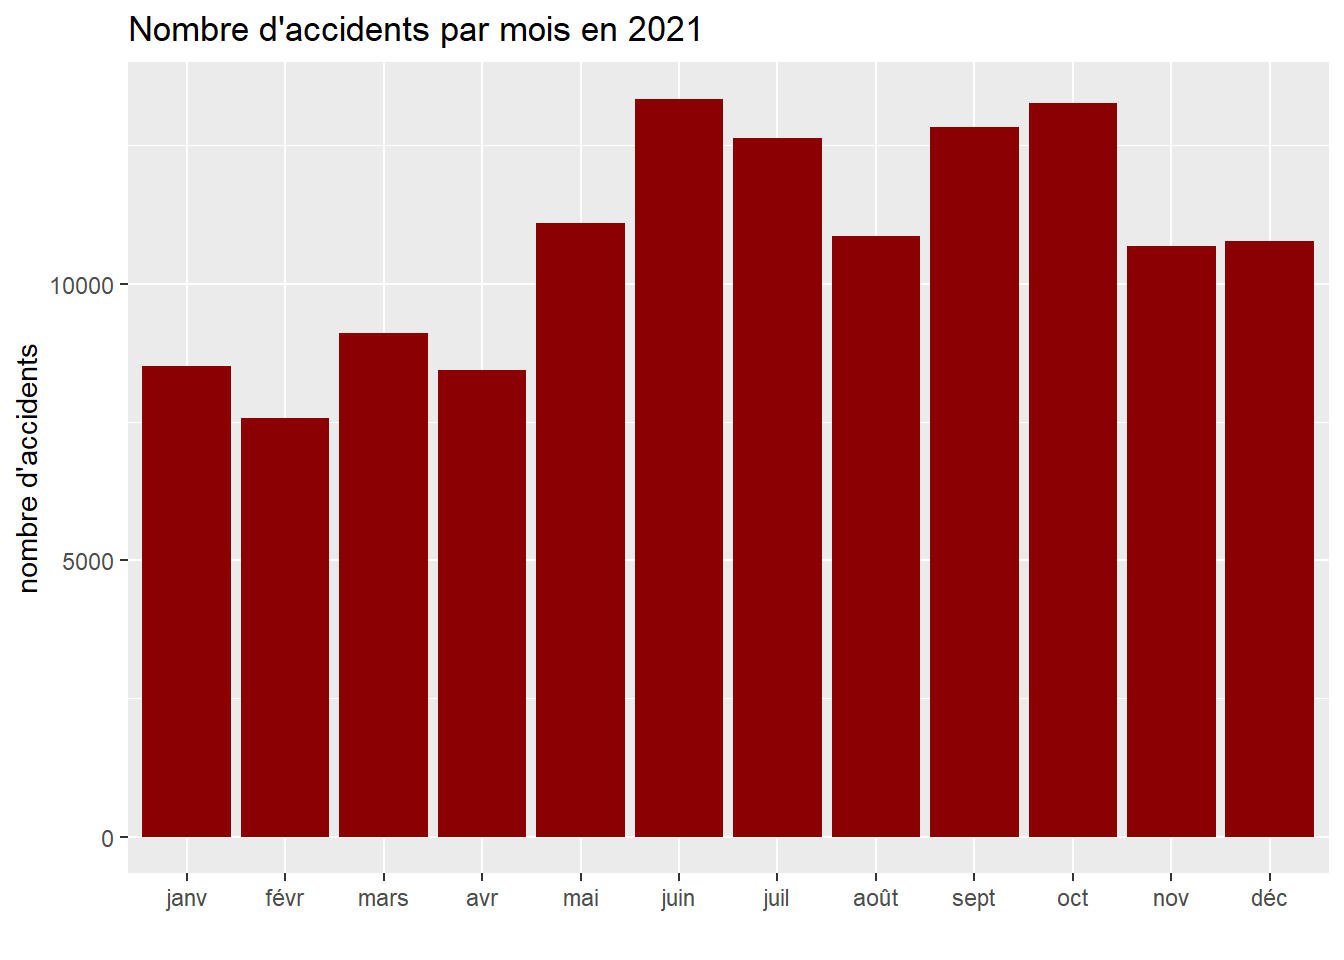
\includegraphics{FLAL_stats_files/figure-latex/pressure-1.pdf}

\hypertarget{tests-plots-sur-les-usagers}{%
\subsection{Tests plots sur les
usagers}\label{tests-plots-sur-les-usagers}}

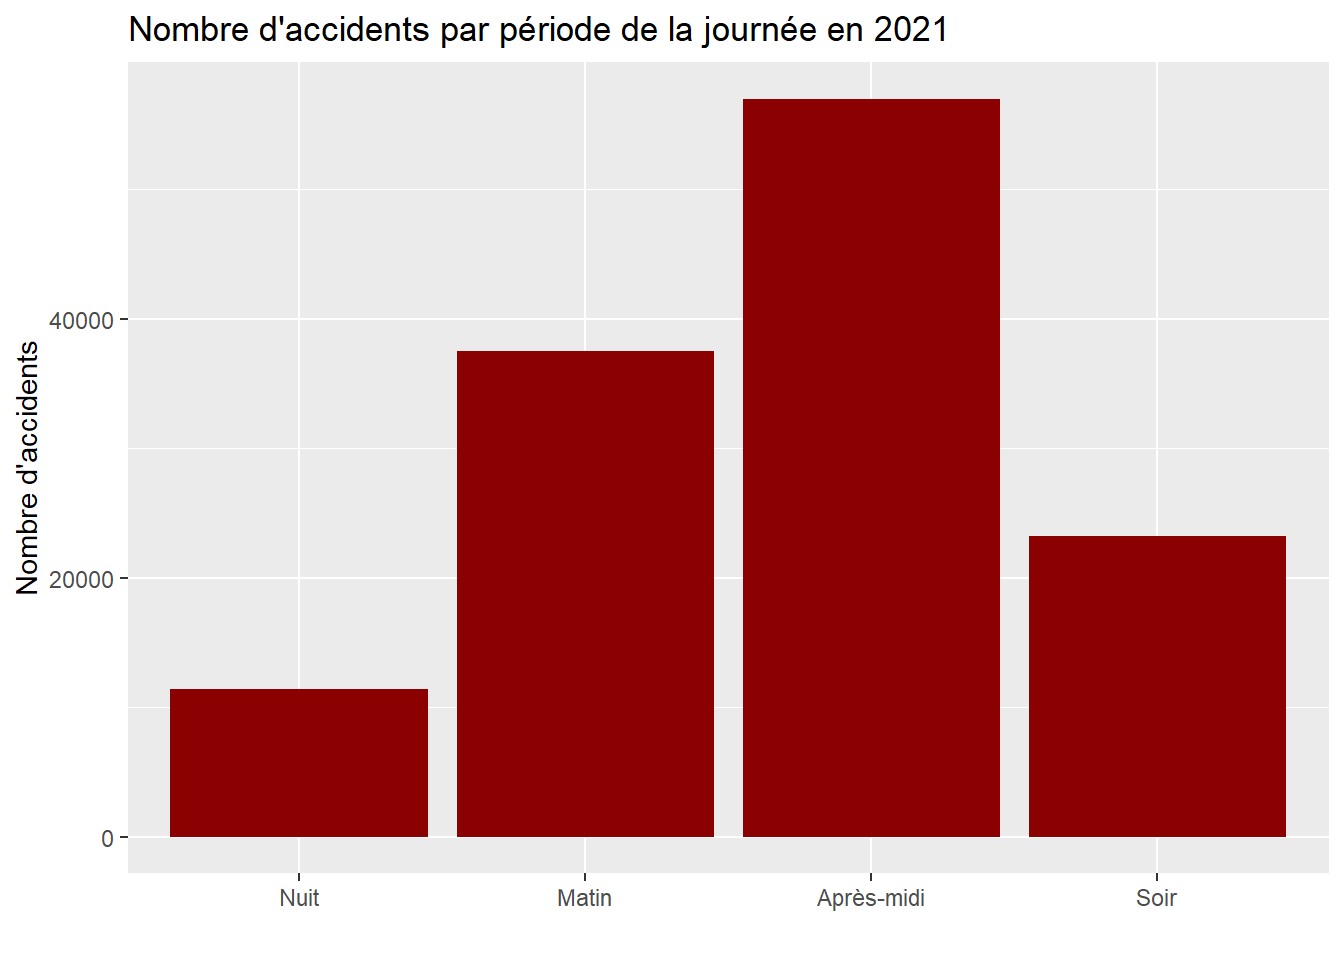
\includegraphics{FLAL_stats_files/figure-latex/unnamed-chunk-2-1.pdf}

\begin{verbatim}
## 
##    -1     1     2 
##  3002 86196 39895
\end{verbatim}

\begin{verbatim}
## Reading layer `regions-version-simplifiee' from data source 
##   `https://raw.githubusercontent.com/gregoiredavid/france-geojson/master/regions-version-simplifiee.geojson' 
##   using driver `GeoJSON'
## Simple feature collection with 13 features and 2 fields
## Geometry type: MULTIPOLYGON
## Dimension:     XY
## Bounding box:  xmin: -5.103601 ymin: 41.36705 xmax: 9.559721 ymax: 51.0884
## Geodetic CRS:  WGS 84
\end{verbatim}

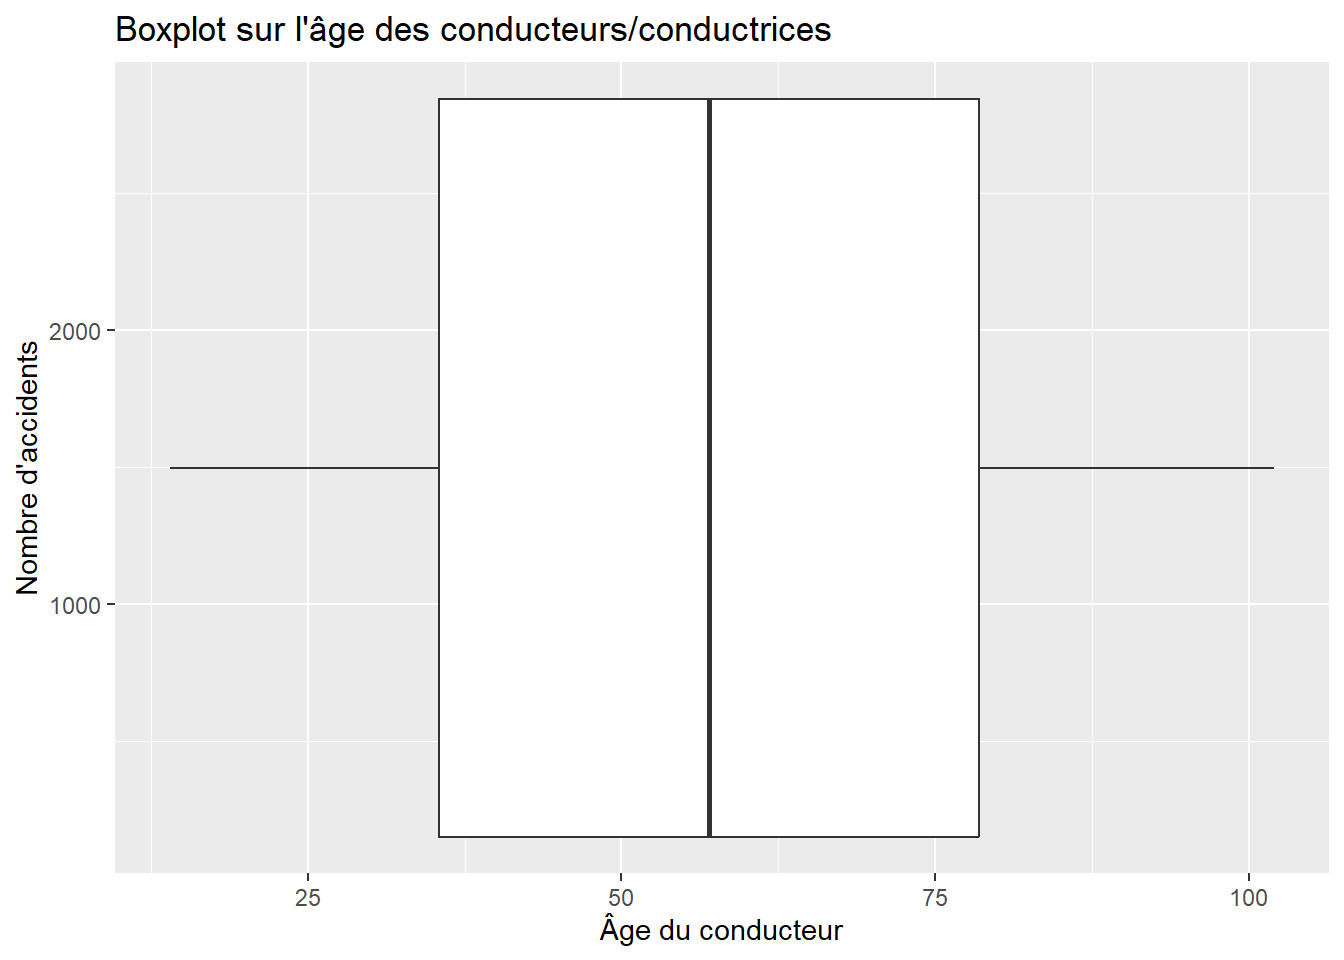
\includegraphics{FLAL_stats_files/figure-latex/unnamed-chunk-3-1.pdf}

\hypertarget{est-ce-que-les-usagers-influencent-la-gravituxe9-des-accidents}{%
\subsection{Est ce que les usagers influencent la gravité des accidents
?}\label{est-ce-que-les-usagers-influencent-la-gravituxe9-des-accidents}}

\begin{itemize}
\item
  Pour les usagers : - on regade nb d'accidents en fonction du sexe
  (pour garder l'esprit féministe) - le nb et la gravité en fonction de
  l'âge
\item
  Pour les véhicules : - on regarde la gravité en fonction du type de
  véhicule (deux roues, voitures classiques etc\ldots) - On regarde la
  gravité en fonction de la sécurité installée pour l'usager (ceinture
  airbag pour les voitures, casque gant veste pour les motards)
\item
  Pour l'environnement : - On regarde la gravité en fonction de la
  vitesse autorisée (en agglo (50km/h)n etc\ldots) - On regarde le nb et
  la gravité en fonction de l'état de la route (mouillée, eneigée,
  sèche) - On regarde le nb et la gravité en fonction de l'éclairage de
  la route (nuit noire, jour, éclairage urbain etc\ldots)
\end{itemize}

\end{document}
